\section{Configuring LAN}

This subsection outlines a pivotal aspect of the internship, detailing the setup and configuration of network infrastructure to facilitate efficient access to the NAS system through a fixed IP address. The integration of a Cisco switch, MikroTik router, and local area network (LAN) aimed to optimize connectivity, data transfer, and seamless user experience.

\subsection{Cisco Switch Configuration}

The configuration process commenced with the Cisco switch, where VLANs (Virtual LANs) were established to segregate network traffic efficiently. Ports were assigned to their respective VLANs based on device types and security requirements. Quality of Service (QoS) settings were fine-tuned to prioritize data traffic, ensuring optimal performance for critical applications.

Key steps in the Cisco switch configuration included:

\begin{itemize}
    \item Creation of VLANs: VLANs were created to logically segment the network, allowing for better control of network traffic.
    
    \item Port Assignment: Each port on the switch was assigned to a specific VLAN, ensuring that devices were placed in appropriate network segments.
    
    \item QoS Configuration: Quality of Service settings were configured to prioritize traffic based on specific criteria such as voice over IP (VoIP) or video streaming, ensuring that critical applications received sufficient bandwidth.
\end{itemize}

\subsection{MikroTik Router Configuration}

The MikroTik router configuration followed, with a focus on establishing secure and efficient routing protocols. Static routes were configured to enable seamless communication between different network segments. Firewall rules were implemented to safeguard the network against unauthorized access, while port forwarding was set up to redirect incoming traffic to the NAS system's fixed IP address.

Key steps in the MikroTik router configuration included:

\begin{itemize}
    \item Static Routing: Static routes were configured to ensure that data packets could travel efficiently between different segments of the network.
    
    \item Firewall Rules: Firewall rules were put in place to control and monitor incoming and outgoing traffic, enhancing network security.
    
    \item Port Forwarding: Port forwarding was configured to redirect external requests to the NAS system's fixed IP address, allowing remote access.
\end{itemize}

For LAN configuration, IP address assignments were managed through Dynamic Host Configuration Protocol (DHCP) to simplify device connectivity. A dedicated subnet was allocated for the NAS system, ensuring consistent communication and efficient data transfer between devices and the NAS.

The success of the configuration was gauged through thorough testing. Network connectivity, data transfer speeds, and NAS access through the fixed IP address were evaluated. Collaborative efforts among team members facilitated troubleshooting and fine-tuning of configurations.

Challenges encountered during the project included optimizing QoS settings for varying network loads, addressing IP conflicts, and ensuring seamless communication between different segments of the network. These challenges were surmounted through meticulous configuration adjustments and collaboration among team members.

The successful outcome of the project resulted in a robust network infrastructure, enabling efficient access to the NAS system through a fixed IP address. This accomplishment demonstrated the significance of effective network design and configuration in facilitating seamless data transfer, optimizing performance, and enhancing user experience.

\subsection{PoE Access Point for Lab Wi-Fi}

In addition to configuring the wired LAN infrastructure, an essential component of our network setup was the utilization of a PoE (Power over Ethernet) access point to provide seamless Wi-Fi connectivity to the lab area. This wireless solution aimed to ensure that both wired and wireless users could access network resources efficiently.

The PoE access point was strategically positioned in the lab area, taking into consideration signal strength and coverage. This access point was chosen for its ability to receive power and data through a single Ethernet cable, simplifying installation and reducing cable clutter.

Key aspects of the PoE access point setup included:

\begin{itemize}
    \item \textbf{Placement and Coverage}: The access point was strategically placed to provide optimal coverage to all lab users. Signal strength and coverage were fine-tuned to ensure a reliable Wi-Fi connection.
    
    \item \textbf{Security Configuration}: Security protocols such as WPA2-PSK (Wi-Fi Protected Access 2 - Pre-Shared Key) were implemented to safeguard the wireless network from unauthorized access.
    
    \item \textbf{Guest Network}: A separate guest network was established to allow visitors to access the internet while keeping them isolated from the internal network resources.
    
    \item \textbf{Quality of Service (QoS)}: QoS settings were applied to prioritize traffic on the wireless network, ensuring that critical applications received adequate bandwidth.
\end{itemize}

The introduction of Wi-Fi via the PoE access point significantly enhanced the flexibility and mobility of lab users. Whether working on laptops, tablets, or smartphones, all users could benefit from a fast and secure wireless connection within the lab environment.

The integration of the PoE access point seamlessly complemented the wired LAN infrastructure, providing a well-rounded networking solution for the lab. It allowed users to access network resources, including the NAS system, from both wired and wireless devices, contributing to the overall efficiency and productivity of the lab environment.
\section{Terminating Cat6 Cables}

The process of terminating Cat6 cables is a critical skill in networking and data communication installations. Proper termination ensures reliable and high-speed data transmission, making it a fundamental aspect of building robust network infrastructures. Termination involves the precise connection of connectors to Cat6 cables' twisted pairs, maintaining signal integrity and minimizing interference.

Terminating Cat6 cables follows industry-standard practices that have evolved to accommodate the demands of modern data networks. Emphasis is placed on maintaining proper cable twists within connectors to prevent signal degradation and crosstalk. Adherence to industry standards defines color codes and pin assignments for consistent terminations.

\begin{figure}[ht]
    \centering
    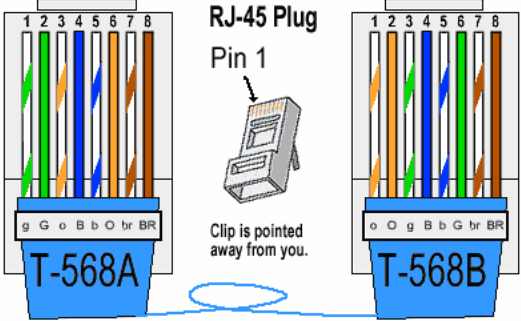
\includegraphics[width=0.6\textwidth]{images/cat6-termination.png}
    \caption{Terminating Cat6 Cable}
    \label{fig:cat6-termination}
\end{figure}

The process typically involves using a crimping tool to cut the cable and attach RJ45 connectors. These connectors securely seal off the individual wires within the cable, ensuring a reliable and secure connection. After crimping, a pair of RJ45 cable testers is employed to confirm a proper connection through the cable before connecting computers or devices to the network switch.

Terminating Cat6 cables requires specific tools and techniques to achieve optimal results. The use of high-quality cable strippers, crimpers, and testers ensures accurate terminations and efficient troubleshooting. Cable testing post-termination to verify continuity and signal quality is essential, ensuring that the cable is ready for deployment.

Moreover, the termination process necessitates attention to detail, precision, and familiarity with the Cat6 cable's structure. Stripping the cable's jacket, untwisting the pairs, aligning the conductors, and crimping the connector are sequential steps that demand meticulous execution.

In summary, the termination of Cat6 cables is a foundational skill for establishing reliable and high-performance network connections. Adherence to industry standards, utilization of proper tools, and meticulous execution, including the use of crimping tools, RJ45 connectors, and cable testers, are vital components of successful terminations that facilitate efficient data transmission and minimal signal interference.
